\documentclass[main.tex]{subfiles}

\begin{document}
\renewcommand{\labelenumi}{\arabic{enumi}.}
\renewcommand*{\phi}{\varphi}

\section{Extremwertprobleme mit Nebenbedingung}
\subsection{Lagrange-Multiplikator}

\section{Extremstellen von Funktionen mit mehreren Veränderlichen}
\begin{enumerate}
    \item Partielle Ableitungen bilden
    \item $\nabla f = \vec{0}$ setzen
    \item $F_y$ nach $y$ umstellen und in $F_x$ einsetzen
    \item Neue Gleichung $0$ setzen und mögliche $x$ Stellen bestimmen
    \item $y$ Koordinaten mit nach $y$ umgestellte Gleichung bestimmen.
    \item Hesse Matrix aufstellen
    \item Punkte jeweils in Hesse-Matrix einsetzen und Definitheit bestimmen
\end{enumerate}

positiv definit => Tiefpunkt\\
negativ definit => Hochpunkt\\
indefinit => Sattelpunkt

Bei einer $\R^{2\times 2}$ Hessematrix:
$D_2 < 0$ -> indefinit. \\
Wenn $D_2 > 0$, $D_1$ bestimmen: Wenn $D_1 > 0$ positiv, wenn $D_1 < 0$ negativ.

\vspace{1cm}

Berechne für jeden Kandidaten $(x_0, y_0)$ die Werte $f_{xx}(x_0, y_0)$, $f_{xy}(x_0, y_0)$ und $f_{yy}(x_0, y_0)$ und daraus den Wert
$$
    d := f_{xx}(x_0, y_0) \cdot f_{yy}(x_0, y_0) - \left(f_{xy}(x_0, y_0)\right)^2
$$
Dann gilt:
$f_{xx}(x_0, y_0) > 0 \ \land \ d > 0 \implies$ \emph{lokales Minimum} \\
$f_{xx}(x_0, y_0) < 0 \ \land \ d > 0 \implies$ \emph{lokales Maximum} \\
$d < 0 \implies$ \emph{Sattelpunkt} \\
$d = 0 \implies$ höhere Ableitung entscheidet \\

\subsection{Hesse-Matrix}
\[
    H_f(x, y) = \eqmatrix{cc}{
        f_{xx} & f_{xy} \\
        f_{xy} & f_{yy}
    }
\]

\section{Stetigkeit}
Ggf. in Polarkoordinaten umwandeln und prüfen, ob ein \textit{winkelunabhängiger} Grenzwert existiert. 
\[
    \lim_{(x,y)\to (0,0)} f(x, y) = \lim_{r\to 0} f(r\cdot \cos\varphi, r\cdot \sin\varphi)
\]
Ggf. lohnt auch eine Betrachtung entlang der Achsen, bspw. bei $x-y$ im Zähler. 

\section{Taylorentwicklung}
Sei $\Delta x = (x-x_0)$, $\Delta y = (y-y_0)$ und $(x_0, y_0) = \vec{\chi}$

\begin{align*}
    T_1(x, y) &= f(\vec{\chi}) + f_x(\vec{\chi}) \cdot \Delta x + f_y(\vec{\chi}) \cdot \Delta y \\[2mm]
    T_2(x, y) &= T_1(x, y) + \frac{f_{xx}(\vec{\chi}) \cdot \Delta x^2}{2} + f_{xy}(\vec{\chi}) \cdot \Delta x \cdot \Delta y + \frac{f_{yy}(\vec{\chi})\cdot \Delta y^2}{2}
\end{align*}
    
    
\section{Vektorfelder}
% grad, rot, div
\subsubsection{Rotation}
\[
    \rot(\vec{v}) = \nabla \times \vec{v} = \vektor{
        \sfrac{\partial}{\partial x} \\
        \sfrac{\partial}{\partial y} \\
        \sfrac{\partial}{\partial z} \\
    } \times \vec{v}
\]
Wirbelfrei wenn $\rot(\vec{v}) = \vec{0}$.

\subsubsection{Divergenz}
\[
    \div(\vec{v}) = \scalarprod*{\nabla, \vec{v}} = \scalarprod*{\vektor{
        \sfrac{\partial}{\partial x} \\
        \sfrac{\partial}{\partial y} \\
        \sfrac{\partial}{\partial z} \\
    }, \vec{v}}
\]
Punkte mit $\div f > 0$ heißen Quellen, $\div f < 0$ heißen Senken des Vektorfeldes.\\
Quellenfrei wenn $\div f = 0$.

\subsection{Potenzialfunktion}
Prüfe ob $\rot(\vec{v}) = \vec{0}$.


\section{Tangentialebenen, Richtungsableitungen}
\subsubsection{Gradient}
\[
    \grad \left(f(x, y)\right) = \nabla f(x, y) = \vector{ f_x(x, y) \\ f_y(x, y)}
\]

Rechenregeln: $f,g: U\to \R$ differenzierbar und $\alpha \in \R$
\begin{align*}
    \nabla (f+g) &= \nabla(f) + \nabla(g) \\
    \nabla (\alpha g) &= \alpha \cdot \nabla(f)\\
    \nabla (f\cdot g) &= g\cdot \nabla(f) + f\cdot \nabla(g) \\
\end{align*}



\subsubsection{Tangentialebene}
\newcommand{\fxxnyn}[2]{
    \textcolor{#1}{
        f_{#2}(x_0, y_0)
    }
}
\begin{align*}
    T(x, y) &=  \fxxnyn{blue!40}{}
    + \scalarprod*{\nabla \fxxnyn{blue!40}{}, (\vec{X} - \vec{X_0})} \\
    &= \fxxnyn{blue!40}{}
    + \fxxnyn{red!70}{x}\cdot (x-x_0)
    + \fxxnyn{orange!70}{y}\cdot (y-y_0) \\
\end{align*}

\[
    T(x, y) = \vector{x_0 \\ y_0 \\ \fxxnyn{blue!40}{}} + \lambda \vector{1 \\ 0 \\ \fxxnyn{red!70}{x}} + \mu \vector{0 \\ 1 \\ \fxxnyn{orange!70}{y}}
\]

\subsubsection{Richtungsableitung}
\[
    D_{\vec{v}}\left(f\left(x_0, y_0\right)\right) = \frac{\partial f}{\partial \vec{v}} = \scalarprod*{\nabla f, \vec{v}} \quad \text{mit} \quad \norm*{\vec{v}} = 1
\]
\subsubsection{Normieren}
\[
    \vec{v} = \frac{\vec{a}}{\norm*{\vec{a}}}
\]
\subsubsection{Richtung des steilsten Anstiegs/Abstiegs}
\[
    \vec{v}_{\text{max}} = \frac{\nabla f}{\norm*{\nabla f}}
    \qquad
    \vec{v}_{\text{min}} = - \frac{\nabla f}{\norm*{\nabla f}}
\]
\subsubsection{Steigung gleich Null}
Orthogonal zur Richtung des Gradienten, also für $\vec{v}_{\text{max}} = \vektor{v_x\\v_y}$ wäre $\vec{v}_{0} = \vektor{-v_y\\ v_x}$ 

\subsubsection{Wert der maximalen Steigung}
\[
    D_{\vec{v}_{\text{max}}}\left(f\left(x_0, y_0\right)\right)
    = \scalarprod*{\nabla f, \vec{v}_{\text{max}}}
    %= \scalarprod*{\nabla f, \frac{\nabla f}{\norm*{\nabla f}}}
    %= \norm*{\nabla f}^{-1} \scalarprod*{\nabla f, \nabla f}
    = \norm*{\nabla f\left(x_0, y_0\right)}
\]

\subsection{Partielle Ableitung}
Eine Funktion heißt partiell differenzierbar, wenn alle partiellen Ableitungen existieren.

\subsection{Vollständiges/totales Differential}
\[
    \dx{z} = f_x (x_0, y_0)\cdot \dx{x} + f_y(x_0, y_0)\cdot \dx{y}
\]

\subsection{Jacobi-Matrix}
\[
    J_f = \eqmatrix{ccc}{
        \frac{\partial f_1}{\partial x} & \cdots & \frac{\partial f_1}{\partial z} \\
        \vdots & \ddots & \vdots \\
        \frac{\partial f_n}{\partial x} & \cdots & \frac{\partial f_n}{\partial z} \\
    }
\]



\subsection{Kurvenintegral}
Kurve/Weg: $\vec{X}: \begin{cases}
    \R &\to \R^n \\
    t &\mapsto \vektor{x_1(t)\\ x_2(t)}
\end{cases}$\\
Ist immer eine Funktion in Abhängigkeit von $t$.\\

Vektorfeld: $\vec{F}: \begin{cases}
    \R^n &\to \R^n \\
    (x, y) &\mapsto \vektor{F_1(x, y)\\ F_2(x, y)}
\end{cases}$

\begin{enumerate}
    \item Wenn nur Punkte gegeben sind: Kurvendarstellung $\vec{X}(t)$ bestimmen
    \item Ableitung der Kurve $\vec{X'}(t)=\vektor{x_1' \\[2mm] x_2'}$
    \item Kurvenpunkte in Vektorfeld einsetzen $\vec{F}\left( \vec{X}(t) \right) = \vec{F}\left( x_1(t), x_2(t) \right)$.
\end{enumerate}
\[
    W = \int_K \vec{F}\dx{\vec{X}} = \int_{a}^{b} \scalarprod*{\vec{F}\left( \vec{X}(t) \right), \vec{X'}(t)} \dx{t}
\]
Tangentenvektor einer Kurve ist $\vec{X'}(t)$.\\
Tangente ist $T(t) = \vec{X}(t) + \lambda\cdot \vec{X'}(t)$.

\subsection{Potentialfunktion}
Sei $\vec{f}: \R^n \to \R^n$. Erfüllt $\vec{f}(x, y)$ die Integrabilitätsbedingung, 
\[
    \frac{\partial f_1}{\partial y} \questeq \frac{\partial f_2}{\partial x}
\]
dann existiert eine Potentialfunktion $V: \R^n \to \R$ mit $\nabla V = \vec{f}$.
\[
    V(x, y) = \int f_1(x, y) \dx{x} = F_1(x, y) + c(y)
\]
$c'(y)$ berechnen mit $\frac{\partial V}{\partial y} \exeq f_2(x, y)$ und Koeffizientenvergleich.\\
Dann $c(y) = \int c'(y) \dx{y}$ in $V(x, y)$ einsetzen. 

\section{Mehrdimensionale Integration}
\subsubsection{Polarkoordinaten}
\[
    \iint f(\textcolor{blue!70}{x}, \textcolor{OrangeRed}{y}) \dx{(x, y)} = \iint f(
        \textcolor{blue!70}{r\cos\phi},
        \textcolor{OrangeRed}{r\sin\phi}
    ) \cdot r \dx{(\phi, r)}
\]
Kreisfläche: $A = \pi \cdot r^2$

\subsubsection{Kugelkoordinaten}
\begin{figure}
    \begin{center}
        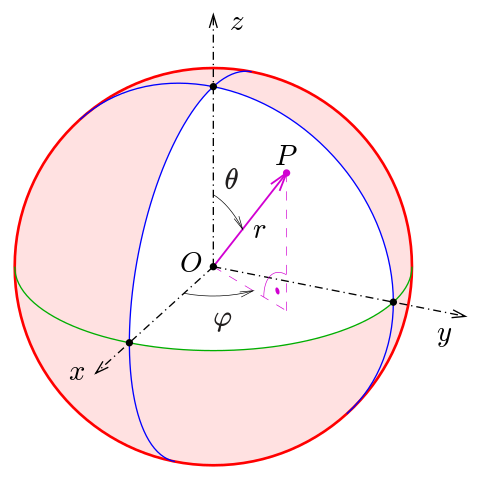
\includegraphics[width=0.5\textwidth]{Kugelkoord-def.svg.png}
        \caption{Kugelkoordinaten. CC-BY-SA by \href{https://commons.wikimedia.org/wiki/User:Ag2gaeh}{User:Ag2gaeh}}
    \end{center}
\end{figure}

\[
    \iiint f(\textcolor{blue!70}{x}, \textcolor{OrangeRed}{y}, \textcolor{OliveGreen}{z}) \dx{(x, y, z)} = \iiint f\left(
        \textcolor{blue!70}{r\cos \phi \sin\theta},
        \textcolor{OrangeRed}{r\sin \phi \sin\theta},
        \textcolor{OliveGreen}{r\cos\theta} \right)
        \abs{r^2 \sin\theta}
        \dx{(\theta, \phi, r)}
\]

Kugelvolumen: $V = \frac{4}{3} \pi\cdot r^3$

\subsection{Schwerpunkte}

\section{Implizite Funktionen}
\begin{enumerate}
    \item $F(x, y)$ nach $0$ umstellen.
    \item Stelle $(x_0, y_0)$ einsetzen und überprüfen ob Gleichung erfüllt.
    \item $F_x$ und $F_y$ bestimmen.
    \item Werte von $F_x(x_0, y_0)$ und $F_y(x_0, y_0)$ ausrechnen.
    \item $y'(x) = - \frac{F_x(x_0, y_0)}{F_y(x_0, y_0)}$
\end{enumerate}


\section{Differenzialgleichungen und Anfangswertprobleme}



\section{Umformungstricks}
\[
	a = \frac{b+1}{b-1} \equiv
	b = \frac{a+1}{a-1}\quad \text{mit } a \neq 1
\]
\[
	a = \frac{b-1}{b+1} \equiv
	b = -\frac{a+1}{a-1} = \frac{a+1}{1-a} \quad \text{mit } a \neq 1
\]

\end{document}
